\documentclass[11pt]{article}
%\usepackage{cite}
\usepackage[numbers]{natbib}
\usepackage{xcolor}
\usepackage{ulem}
\usepackage{graphicx}
\usepackage{subcaption}
\usepackage{multirow}
\title{\textbf{Draft research question}}
%\author{Mathias Parisot}

\begin{document}
\maketitle

\section{Roadmap}

\begin{enumerate}
  \item introduction and literature study (1.5 weeks) introduction + related works
  \item draft methodology to answer research question (1 week)
  \item \textbf{experiment with simple attacks (1-2 weeks)}
  \item \textbf{implement methodology and start experiment (3-4 weeks)}
  \item analyse results (2-3 weeks)
  \item write paper (2 weeks)
  \item presentation(1-2 weeks)
\end{enumerate}

\section{Research question}

    Machine learning applications have grown in popularity over the last decade. One of the most used kinds of models are neural networks which grew in popularity with the advances in hardware and deep learning algorithms, and because they excel in image recognition and natural language processing applications. Cloud providers have included Machine Learning as a Service to their offer, it is now easier than ever for businesses to deploy machine learning models. MLaaS platforms such as AWS\footnote{https://aws.amazon.com/machine-learning/}, Microsoft Azure\footnote{https://azure.microsoft.com/en-us/services/machine-learning/}, Google Cloud AI\footnote{https://cloud.google.com/ai-platform} or IBM Watson\footnote{https://www.ibm.com/cloud/machine-learning} offer their customers to train their model given they provide the dataset. \textcolor{red}{The final model is then shared or can be accessed through queries. However, such models, and machine learning models in general, are sensitive to malicious attacks. The attacks can impact the privacy of the training set, or the well-Extraction attacks aim at infering the architecture and the parameters of the attacked model to create a duplicate. Inversion attacks aim at infering information from the data the attacked model was trained on. Data poinsoning and adversarial attacks aim at compromising the attacked model predictions either by polluting the training data, or by crafting malicious inputs to feed into the model.
    \sout{The final model can be queried as a black-box or not, it is nevertheless sensible to privacy attacks aiming at inferring information from the data it was trained on.}}.\\
    \textcolor{red}{Several kind of model inversion attacks exist with different goals: the attacker could want to determine whether a data instance was used for training (membership inference)\cite{Shokri2017, Salem2019}, reconstruct a representative of a particular class of the training set \cite{Fredrikson2015}, or infer hidden properties of the training set (property inference)\cite{Ganju2018}. \sout{Privacy attacks can go from determining whether a data point was used for training,  (\textit{membership} inference), reconstructing class representatives (\textit{model inversion}), or inferring hidden properties of the training set (\textit{properties inference})}}\\
    
    (TO DO): The implementation of the GDPR in 2018 has put a question on whether those kinds of models are compliant (\textcolor{red}{\textit{\underline{question}: can it be argued that if the model learns more information than it needs, then Art.5.1.c - data minimization applies?} I still need to write this part}).\\
    
Membership inference attacks work the following way: given a data point, determine whether it was used to train the given model. The issue with such attacks is they are not always applicable in real-life settings as the attacker needs to get a copy of one of the training data before determining whether it belonged to the training set. Inversion model attacks operate such that, for a classifier, for example, a class representative can be created. While they are impressive for face recognition models, they only build the “average” representation of the class and do not work well if the data instances are not similar.
Property inference attacks (PIA) aim at inferring properties learned by the model that are independent of the characteristics of the class the model is trained to recognize. There have been fewer studies on this kind of attack, \textcolor{red}{according to \citet{He2019} only 4 papers were published on model inversion attacks against 10 for membership inference attacks. \sout{according to \cite{He2019} they only account for 28\% of the published papers on model inversion attacks agains 72\% for membership inference attacks}}. In \cite{Ganju2018} the authors identify the invariance of fully connected neural networks to node permutation as a limiting factor of PIA efficiency and show that using a Deep Set architecture \cite{zaheer2017deep} is an effective way to tackle this limitation. In \cite{Melis2019} the authors successfully perform PIA in a collaborative learning setting where the attacker is one of the members.\\

The kind of model used has an impact on the kind of attacks that can be used on it (\textcolor{red}{I still need to do that. \textit{\underline{remark}: I probably need to include a source here, it is a bit of a strong claim.}}). As computer vision and natural language processing popularity increases, more complex neural network architectures are created even if their vulnerability to privacy attacks is still not fully determined \cite{He2019}. None of the current work studied the relationship between the depth and width of a deep neural network and its sensibility to PIA. \citet{Geiping2020} analyzed the effect of model architecture on sensibility to model inversion attacks on non-sensible data (cars, animals).\\


\textbf{In case of a trained Neural Network, are sensitive properties of the underlying dataset at risk due to property inference attacks, and if so, how does that risk relate to the architecture of the model such as depth and width?}
\begin{itemize}
\item{\textcolor{red}{How does the sensibility to property inference attacks change with changes in depth and width of deep neural networks?}}
\item{\textcolor{red}{Does it affect compliance to the GDPR with respect to processing of sensitive data?}}
\item{\textcolor{red}{Question: do I still need to specify the secondary questions when the initial research qeuestion is detailed? Or should I make the research question broader and the secondary questions more detailed?}}
\end{itemize}

\section{\textcolor{red}{Background}}

\subsection{\textcolor{red}{Deep Learning model}}
(TO DO)
\subsection{\textcolor{red}{Federated Learning}}
(TO DO)
\subsection{Property Inference Attack}

The main idea of a PIA is to train an attack model $M_a$ which takes as input a trained model and outputs the probability that $P$ is true for the training set of the input model. Once the attack model is trained, the attacker can give it the target model $M_t$ as input and know whether the $P$ is true for the dataset used to train the target model. To train $M_a$, the attacker uses several shadow models ($M_{s1}$ ... $M_{sk}$) which are respectively trained on datasets $D_1$ ... $D_k$ specifically crafted by the attacker to contain or not the target property $P$. Once the shadow models are trained, they are used as the training set for $M_a$. The general overview of the attack is described in Figure \ref{pia_diagram}.\\
%The datasets $D_1$ ... $D_k$ are generated using data synthesis.

\begin{figure}[h]
    \centering
    \begin{minipage}{\textwidth}
        \centering
        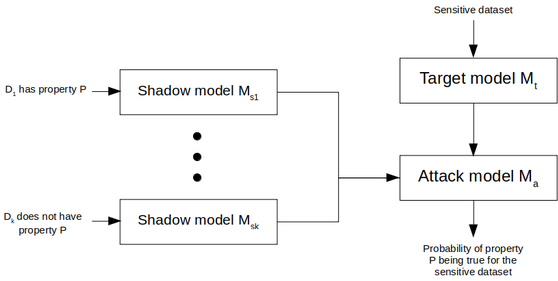
\includegraphics[width=0.99\textwidth]{pia_diagram2.png} % first figure itself
        \caption{Property Inference Attack using shadow models.}
        \label{pia_diagram}
    \end{minipage}\hfill
\end{figure}

\section{Methodology}

\subsection{Threat model}

We assume the target model is a deep neural network trained for a classification task on a sensitive dataset containing personal data. The attacker has access to the full architecture and parameters of the model (white-box setting). While a white-box model facilitates the job of the attacker, it is reasonable as it is common in some machine learning paradigms such as Federated Learning \cite{shokri2015privacy} where the clients, and sometimes the server, have full knowledge of the model. \textcolor{red}{Moreover, model extraction attacks have been performed with close to perfect performance, converting the black-box setting into a white-box one \cite{DBLP:journals/corr/PapernotMGJCS16}. How the attacker manage to obtain the weights and the architecture of the model is out of the scope of this study. \sout{There also exists model extraction attacks with close to perfect performance \cite{DBLP:journals/corr/PapernotMGJCS16}}}. The goal of the attacker is to infer general information about the training dataset. Such information could be the proportion of the training data having a property unrelated to the main classification task of the model.

\subsection{Datasets}

CelebFaces Attributes (CelebA) \cite{liu2015faceattributes} is a face attributes dataset containing more than 200 000 images of more than 10 000 celebrities taken from online. The images are labeled using 40 physical attributes such as hair color, smiling, wearing a hat. We use the dataset to train model $M_t$ to detect whether the person is wearing glasses.
To add other datasets if we end up using more.\\
25 different architectures of target models are trained using 5 width and 5 depth values. The width values are 8, 16, 32, 64, 128 (\textit{\underline{to add}: I don’t know what reasonable width values to use at the moment}). The depth values are 10, 20, 40, 80, 160 (\textit{\underline{to add}: same, I am not sure what values yet. I saw 18, 20, 110 in \cite{Li2020} but it was not for face attributes detection}). The list of the architectures and their test accuracy is presented in the table 


\begin{table}[]
\centering
\begin{tabular}{cl|l|l|l|l|l|}
\cline{3-7}
\multicolumn{1}{l}{}                         &     & \multicolumn{5}{c|}{depth} \\ \cline{3-7} 
\multicolumn{1}{l}{}                         &     & 10  & 20  & 40  & 80 & 160 \\ \hline
\multicolumn{1}{|c|}{\multirow{5}{*}{width}} & 8   &     &     &     &    &     \\ \cline{2-7} 
\multicolumn{1}{|c|}{}                       & 16  &     &     &     &    &     \\ \cline{2-7} 
\multicolumn{1}{|c|}{}                       & 32  &     &     &     &    &     \\ \cline{2-7} 
\multicolumn{1}{|c|}{}                       & 64  &     &     &     &    &     \\ \cline{2-7} 
\multicolumn{1}{|c|}{}                       & 128 &     &     &     &    &     \\ \hline
\end{tabular}
\caption{Target models accuracies on CelebA.}
\label{pia_diagram}
\end{table}
\subsection{Evaluation}

The two properties we try to infer are both sensitive according to the GDPR and are listed as follow:
\begin{itemize}
  \item $P_1$: whether the training set contains an imbalanced number of male/female (\textit{\underline{question}: maybe infer the exact proportion is a more impressive feat, it is probably more difficult})
  \item $P_2$: whether the training set contains an imbalanced number of light skin celebrities
\end{itemize}
\textit{\underline{to add}: I want to describe which metrics I'm going to use to assess the attack.}


%\renewcommand\bibliographytypesize{\small}
%\bibliographystyle{alpha}
%\bibliography{references.bib}{}
\bibliographystyle{unsrtnat}
\bibliography{references.bib}


\end{document}
